\subsection{Architettura generale}

\subsubsection{Schema}
\begin{figure}[H]
    \centerfloat
    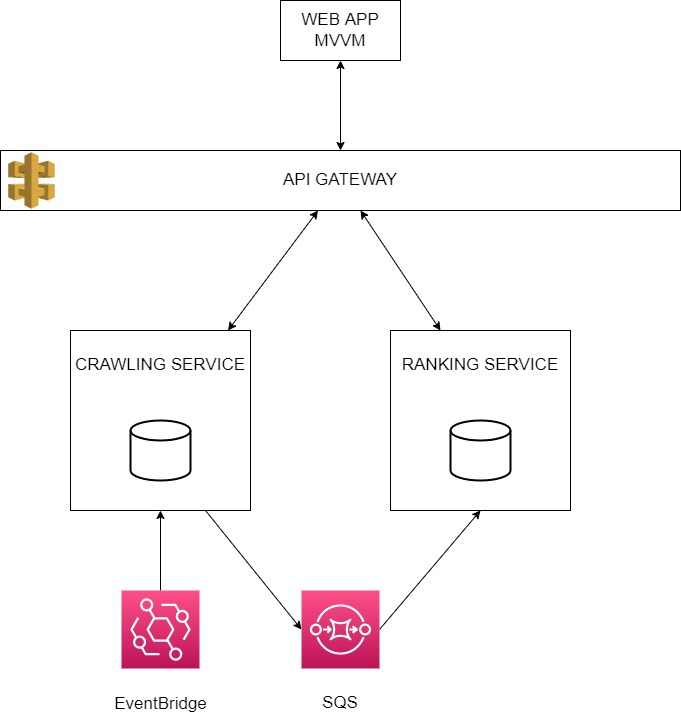
\includegraphics[scale=0.35]{Contenuto/Immagini/backend-architettura.jpg}
    \caption{Architettura generale}
\end{figure}

\subsubsection{Descrizione}
Come richiesto dal capitolato si è deciso di utilizzare un'architettura a microservizi, i quali comunicano con il frontend tramite API gatewaty.
In particolare sono stati individuati i seguenti microservizi:
\begin{itemize}
    \item \textit{Crawling Service}: questo microservizio si occupa di tutto ciò che riguarda il crawling dei dati da instagram. Il processo di crawling viene innescato da un servizio di AWS chiamato EventBridge che si occupa dello scheduling del crawling. Ogni volte che viene trovato dal crawler un post relativo ad un ristorante, questo viene inviato ad una coda di tipo SQS dalla quale andrà a leggere il servizio di ranking. Infine il Crawling Service espone una API al frontend per permettere di suggerire profili instagram da aggiungere alla lista di quelli osservati dal crawler.
    \item \textit{Ranking Service}: questo microservizio invece si occupa dell'analisi dei contenuti estratti dal crawler e della realizzazione di una classifica di ristoranti. Il processo di analisi di un post viene fatto partire dalla ricezione di un messaggio sulla coda SQS, una volta letto il messaggio esso viene rimosso dalla coda ed analizzato. Infine il Ranking Service espone molteplici API al frontend in grado di fornire tutte le informazioni necessarie per poter visualizzare la classifica, i dettagli di un locale e la gestione dei preferiti.
\end{itemize}
Il frontend infine adotta un pattern MVVM e comunica col backend esclusivamente tramite API gateway. Grazie al servizio di AWS chiamato Cognito, tutta la parte relativa all'autenticazione è gestita lato frontend.